\documentclass[output=paper,
modfonts
]{langscibook} 
\bibliography{localbibliography}

\usepackage{tabularx,multicol}
\usepackage{url}
\urlstyle{same}

\usepackage{longtable} % to be able to make the long table in Data span over multiple pages - JP
\usepackage{multirow} % to be able to use the multirow command - needed for Paper 2 tables

\usepackage{langsci-lgr}
\usepackage{langsci-branding}
\usepackage{langsci-optional}
\usepackage{langsci-gb4e}


\makeatletter
\let\thetitle\@title
\let\theauthor\@author
\makeatother

\newcommand{\togglepaper}[1][0]{
%   \bibliography{../localbibliography}
  \papernote{\scriptsize\normalfont
    \theauthor.
    \thetitle.
    To appear in:
    Change Volume Editor \& in localcommands.tex
    Change volume title in localcommands.tex
    Berlin: Language Science Press. [preliminary page numbering]
  }
  \pagenumbering{roman}
  \setcounter{chapter}{#1}
  \addtocounter{chapter}{-1}
}

\newcommand{\bari}{\ipabar{\i}{.5ex}{1.1}{}{}}
\newcommand{\notipa}[1]{\textnormal{#1}}

\newcommand{\agre}{\textsc{agr}-\ol{eene}}

\renewcommand{\emph}[1]{\textit{#1}} % resetting a setting from ling-macros-modified (I think?)

% forest settings to make compact but (mostly) straight-spined trees:
\forestset{
fairly nice empty nodes/.style={
            delay={where content={}{shape=coordinate,for parent={
                  for children={anchor=north}}}{}}
, angled/.style={content/.expanded={$<$\forestov{content}$>$}}
}}

\forestset{sn edges/.style={for tree={parent anchor=south, child anchor=north}}}

\newcommand{\bex}{\begin{exe}}
\newcommand{\fex}{\end{exe}}

\newcommand{\bxl}{\begin{exe}}
\newcommand{\fxl}{\end{exe}}

\newcommand{\ix}[1]{\textsubscript{#1}}
\newcommand{\alert}[1]{\textbf{#1}}
\newcommand{\ol}[1]{\textit{#1}}


\newenvironment{context}{\begin{quote}%
			\bfseries Context: \\%
			\mdseries\slshape }%open environment
			{\end{quote}}%close environment




			\usetikzlibrary{shapes,arrows,positioning,decorations,decorations.pathmorphing,intersections}
\forestset{
nice empty nodes/.style={
    for tree={calign=fixed edge angles},
    delay={where content={}{shape=coordinate,for siblings={anchor=north}}{}}
},
}

\definecolor{dark-gray}{gray}{0.3}

%\usepackage{dingbat,pifont}


%%%%%%%%%%%%For arrows%%%%%%%%%%%%%

\newcommand\Tikzmark[2]{%
  \tikz[remember picture]\node[inner sep=0pt,outer sep=0pt] (#1) {#2};%
}
\NewDocumentCommand\DrawArrow{O{}mmmmO{3}}{
\tikz[remember picture,overlay]
  \draw[->,line width=0.8pt,shorten >= 2pt,shorten <= 2pt,#1]
    (#2) -- ++(0,-#6\ht\strutbox) coordinate (aux) -- node[#4] {#5} (#3|-aux) -- (#3);
}
\NewDocumentCommand\DrawDotted{O{}mmmmO{3}}{
\tikz[remember picture,overlay]
  \draw[->,line width=0.9pt,dotted,shorten >= 2pt,shorten <= 2pt,#1]
    (#2) -- ++(0,-#6\ht\strutbox) coordinate (aux) -- node[#4] {#5} (#3|-aux) -- (#3);
}
\NewDocumentCommand\DrawLine{O{}mmmmO{3}}{
\tikz[remember picture,overlay]
  \draw[line width=0.8pt,shorten >= 2pt,shorten <= 2pt,#1]
    (#2) -- ++(0,-#6\ht\strutbox) coordinate (aux) -- node[#4] {#5} (#3|-aux) -- (#3);
}
%%%%%%%%%%%%%%%%%%%%%%%%%%%%%%%%%%%%%


\newcommand{\baru}{ʉ}
\newcommand{\baruH}{\'\baru}
\newcommand{\baruL}{\`\baru}

\newcommand{\ep}{ε}
\newcommand{\epH}{\'\ep}
\newcommand{\epL}{\`\ep}

\newcommand{\schwa}{ə}
\newcommand{\schwaH}{\'ə}
\newcommand{\schwaL}{\`ə}

\newcommand{\oo}{ɔ}
\newcommand{\ooH}{\'\oo}
\newcommand{\ooL}{\`\oo}

\newcommand{\ds}{\ꜜ}

\newcommand{\ch}{t͡ʃ}
\newcommand{\dz}{d͡ʒ}

\newcommand{\tgl}{ʔ}

%shortcuts for the complementizers
\newcommand{\mbuL}{mb\baruL}
\newcommand{\mbuHL}{mb\baruH\baruL}
\newcommand{\mbuLH}{mb\baruL\baruH}
\newcommand{\la}{lá}
\newcommand{\nda}{ndà}

\newcommand{\tsc}[1]{\textsc{#1}}
\renewcommand{\textscb}{ʙ}
\newcommand{\ipa}[1]{#1} %disable IPA

 
\title{Language Shift}  

\author{%
 Andreia Caroline Karnopp\affiliation{University of Zurich}
}

% \chapterDOI{} %will be filled in at production
% \epigram{}

\abstract{
Language Shift has always existed. Conquests were the first cause of language shifts, then migrations prompted these types of changes, and today it is mainly language diffusion that triggers this language contact phenomenon. There are some promoting and/or retarding factors for shift, but not a single condition evokes the same patterns of language use in all language contact situations. For this reason, and because each language community should thus be considered and analyzed in isolation, this chapter discusses the most significant approaches, models, methods and examples of possible language choice patterns and trends, and finally, also addresses possible factors that may or may not boost language shift within a determined linguistic community.
}

\begin{document}
\maketitle

\section{Introduction}

Since \emph{Language Shift} (LS) is always preceded by language contact or collective multilingualism \parencite[320]{Ostler2011}, this social phenomenon is important to include in the discussions addressed within this book. Even if LS can happen at an individual level (\emph{Language Attrition} (LA)\footnote{LA is about ‘forgetting' an educational or extracurricularly learned L1, L2 or foreign language. It thus describes the loss of language skills by an individual and can in a way be considered as a reversal of language acquisition \parencite{Lambert1982}.}), it usually refers to the change in usage of a given language community from a language A to a language B in all situations and domains. This change in norm is usually observable as a bi- or multilingual period within one or across several generations.

LS is often described as a kind of `transitional phenomenon' \parencite[33]{Bohm2010} of changing language contact situations. It refers to a shift away from a `healthy' language state due to a `disorder' or a range of `disorders'\footnote{The term ‘disorder(s)' here refers to the fact that a previously rather stable speech contact situation -- above described as ‘healthy' -- can become unstable and cause a ‘disorder' as a result of various mostly related factors, and therefore change the habitual language use (clearly visible in stage B of Figure \ref{figure1} ).} of the affected languages. \emph{Language maintenance} (LM), in contrast, describes a relatively stable\footnote{LM is described here as ‘relatively stable', since long-lasting and intensive language contact can lead to interferences (e.g. borrowing-scale by \citealt{thomasonkaufman1988}), and further language contact phenomena.} language contact situation in which bilingual speakers, speaker groups or an entire linguistic community continue using the minority or heritage language\footnote{Alternative terms used in the literature are community language, (im)migrant language, ethnic language, and home language. Heritage language, however, is probably the most widely used term \parencite[23]{Pauwels2016}.}, despite the pressure of the majority and socially dominant language and other influencing factors. Consequently, the mentioned `disorders' can provoke different patterns of language use, which is why each language contact situation must be considered separately. What all situations have in common, however, is that LS affects only groups and communities which are in contact with a more dominant and more powerful social group. This is why LS is generally understood as ‘a barometer of inequality between linguistic minorities and the majority’ \parencite[613]{Heinrich2015}.

LS is not a recent phenomenon, but has been occurring throughout the history in different societies and in diverse places \parencite[4]{Puthuval2017}. \cite[326-328]{Ostler2011} supposes that LS started happening with the Neolithic revolution and the related establishment and settlement of humankind -- however, it can be assumed that these processes were already taking place before this period. Between 3000 BC and 1500 AD, dominant languages spread mainly through \emph{wars} and subsequent \emph{conquests} of rural societies. Since then, the languages of European conquest have prevailed -- e.g. Spanish in Latin America, Portuguese in Brazil or English in the USA. Dominant languages are therefore often associated with oversea explorations, invasions and migrations. Before the 20th century, \emph{migration} was the biggest risk for a group to be affected by LS. Nowadays, in contrast, the physical \emph{diffusion}\footnote{\emph{Language diffusion} (LD) often happens on an individual level and is promoted by e.g. \emph{cohabitation} (founding bilingual families) or by \emph{recruitment} (new employment, military, etc.) \parencite[323-324]{Ostler2011}.  In certain domains a LS can then progress quickly and widely. \emph{Linguistic diffusion}, on the other hand, refers to a shift of individual linguistic variants within a language -- which can also be caused by language contact -- on an individual or social level over a longer period of time. Both speakers and listeners can give different preferences to individual variants or even generate new variants \parencite{Gong2012}.} of so-called world languages plays an increasing role because young people tend to learn one of these rather than maintain their parents' minority language. 
\begin{figure}
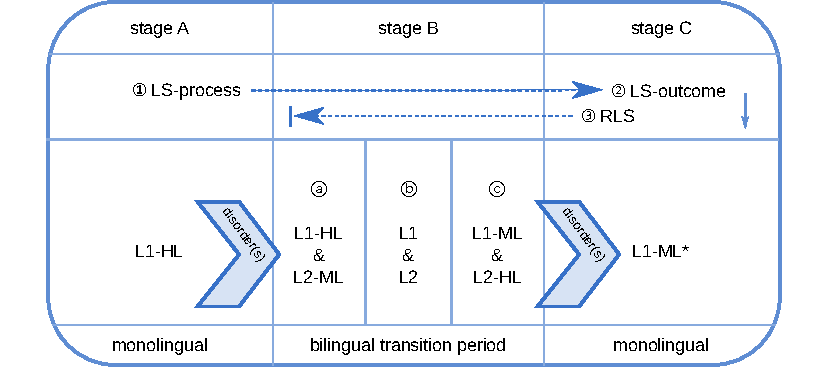
\includegraphics[width=10cm]{Karnopp_pic1}
\caption{\emph{Language Shift Model}Abb.: L1 = first
  language; L2 = second language; HL = heritage language; ML = majority
  language; L1-HL = abandoned/heritage language; L1-ML* =
  target/majority language (can contain phonetic, morphologic,
  syntactic, semantic and prosodic traces from the HL.}
\label{figure1}
\end{figure}

%Both figures (Fig 1 and 2) were created by me especially for this chapter. How can I quote that?

As most of the LS literature, this chapter will mainly discuss the language use of minority groups -- migrant communities and territorial linguistic minorities, with a special focus on the former. Therefore the model in Figure \ref{figure1}, which is based on \cite{Fishman1964}'s three-generational model, illustrates the different phases typically leading to LS in migrant groups. Likewise \cite{Weinreich1953} assumes that at least three generations are necessary for LS to happen. \cite[6]{Ortman2008}, in contrast, point out that in many \emph{inter}generational analyses, the so-called `mother tongue shift' occurs mainly in the second and third generation. In this regard, LS can be understood here as a gradual and progressive process ① or as a reversible process ③ of the dynamics of a natural multilingual language community. On the other hand, LS is sometimes also analyzed as an outcome ② or a consequence of a language contact situation: The use of the languages changes across the three stages in Figure \ref{figure1}. A monolingual stage A is followed by a situation of language contact, caused, for instance, by migration. A bilingual transition period then follows, which is often \emph{diglossic}\footnote{\emph{Diglossia} is a special form of bilingualism of a language community in which a high and a low variety coexist. While \cite{Ferguson1959} distinguished between two variants of the same language (e.g. the case of German and Swiss German in the German-speaking part of Switzerland), \cite{Fishman1967} extended this definition to language contact situations of unrelated varieties (e.g. Hindi and Tamil in India).} and in which the collective language choice is \emph{variable} \parencite{Fasold1984}. This middle stage, which is at the heart of the progressive LS process ①, can last for one or more generations, and may affect an entire language community as follows. Three different types of bilingualism are distinguished for stage B: ⓐ supplementary, ⓑ complementary  (see LM), and ⓒ replacive bilingualism \parencite{Haugen1972}. Given that the preferred language can influence the language skills of every individual speaker (in LS situations the L1-HL, and in RLS situations the L1-ML), the three types of bilingualism can also co-occur within the same community. The bilingualism phase is then followed by another not necessarily purely monolingual stage C, as Fishman \parencite*{Fishman1964} idealistically showed. The target language can still contain traces of the L1-HL in the form of code mixing or code switching (see \emph{shift variety} in Section \ref{patterns}, and Chapter 3), 
%Crossreference
or even adopt new features from the heritage language and thus end up in a new variety or language (see Chapter 4).

\subsection*{LS as outcome ②}

Languages are social entities that need an associated society in order that their memory not be lost. This means that if speaker groups or societies, for example migrants, do not live in their home countries and lose contact with them, there is a good chance that they will shift more quickly to the L1-ML. Therefore, a language's survival depends on who speaks what, to whom and when \parencite{Fishman1964}.

The \emph{transmission} of an L1-HL to the following generations can be disturbed or inhibited during the three LS phases (see Figure \ref{figure1}) for various reasons, e.g. if a language community dies out, if it is conquered by another group who speaks a different language, or if it is eradicated (see Chapter 4)\footnote{It is important that we take into account here that LS does not end with a person's life or the life of a group, but rather represents a shift or a change from generation to generation \parencite[195]{Jagodic2011}.}. The speakers make or are forced to make a so-called ‘social choice' in order to better integrate themselves (or not) in the new society \parencite[325]{Ostler2011}. In other words, the preference for one of two or more contact languages automatically generates social closeness or distance. So if a bilingual speaker chooses the L1-ML, he automatically selects social proximity to the out-group and social distance to the in-group -- and vice versa. At this point in time the corresponding L1-HL is threatened if it is not spoken by another group or if it is not used for a specific purpose there is danger of becoming an \emph{endangered language}\footnote{Without adequate documentation, frequent use between L1-HL speakers in different situations and domains, and without transmission to the next generation, a language is \emph{endangered} and thus threatened with extinction (see EGIDS, the 13 levels of language endangerment/vitality proposed by \cite[2]{Brenzinger2003} based on Fishman's (\citeyear{Fishman1991}) 8-level GIDS -- see Section \ref{approaches}.}. The former mother tongue is then gradually replaced from generation to generation by the L1-ML (\emph{obsolescence} or \emph{language dead} at group level and \emph{attrition} at speaker level, e.g. \citealt{Crystal2000}).
According to \cite[7]{Nettle2000}, more than half of the more than 6000 languages spoken in the world are currently at such a stage. The process mainly affects small minority languages in Australia, the Pacific and in North and South America. Normally, such an advanced state of LS is irreversible, and has therefore achieved its \emph{morbid endpoint}\footnote{The difference between a \emph{morbid endpoint} of a language and \emph{language death} is that in the former case a language can still be spoken by other language communities.  On the other hand, the term \emph{language death} can be understood literally, because in this case a language is not spoken anymore, because it has been forgotten or simply not learned or passed on, and therefore no longer exists.} -- and not \emph{death} \parencite[18]{Pauwels2016}.


\subsection*{Reversing LS ③}

If a speech community sees a reason to take active steps to preserve an endangered (heritage) language, and if the language policy of a region or country supports these actions, an \emph{ongoing}\footnote{LS is to be viewed as a process in which different factors come together. This can be extremely dynamic. For this reason, and so that a model can be predictable at all, it must be flexible and able to take account of changing circumstances. Therefore I use the term \emph{ongoing}, like \cite[112]{Pauwels2016}.} LS-process can change direction and be reversed (\emph{Reversing Language Shift}, RLS), if it has not yet reached the \emph{morbid endpoint}. The heritage language can be documented by linguists and stored in archives, or get actively preserved and maintained through revitalization \parencite[315]{Ostler2011}. This reversal requires a new distribution of power between the language communities, which may lead to a different language policy issue. The idea of many supporters of minority languages is to teach it to the younger generation in school so as to enable them to use it regularly and pass it on to subsequent generation(s) \parencite[4]{Puthuval2017}. If an L1-HL plays a part in defining a sense of identity (see \emph{core-value}), if it hosts the community's culture and traditions, and if it is the basis of knowledge and experience, nowadays people or institutions often eagerly try to preserve that language. In this respect, language diversity, even though LS is the social norm \parencite[84]{Pauwels2016}, is still a universal phenomenon.

\subsection*{LS-process ①}

On the other hand, LS can also be understood as a process, process in the sense that  the dominant language spreads at the cost of the minority language \parencite[31]{Bohm2010}. Language `lives' and is associated with an \emph{ongoing} learning process that can lead to changes such as
variant formation (see Chapter 2, short- or long-term-accommodation),
%Crossreference
speaker-related language mixing (see Chapter 3, code-switching), 
%Crossreferencenew
new languages or varieties (see Chapter 4, Creoles and Pidgins) 
%Crossreference
and thus to long-term change (language shift or language change). Due to differences in individual settings, situations, speakers, etc., there is still \emph{no uniform and general definition} of the phenomenon LS. As \cite[19]{Pauwels2016} explains:

\begin{quote}
it may take one or more generations of speakers before the language is entirely abandoned. It also implies that the shifting away from the L1 does not occur simultaneously across all its users or functions and settings. The rate and speed of the shift process will vary from community to community. In some cases the process is relatively swift, within one or two generations, and in other contexts it will take much longer.
\end{quote}

The duration of the shift process therefore depends on various influencing factors (see Section \ref{factors}): While some language communities change their main language within only one generation, for instance, Dutch migrants in New Zealand (e.g. \citealt{VanRijk2017}), other migrant groups manage to maintain their L1-HL over several decades or centuries as the Amish  in the USA (e.g. \citealt{Sağlamel2013}) or the Swiss in Brazil (e.g. \citealt{Karnopp}).

Figure \ref{figure1} represents an overview of the phases typically involved in LS in a bilingual language community with language contact. However, this model does not hold for all settings and all contact situations with LS as an outcome. The transition period between a monolingual setting with language A and a monolingual setting with language B can be more multifaceted than depicted in Figure \ref{figure1} . The transition phase is discussed in more detail in the following subsections. Section \ref{approaches} discusses the main approaches to LS, presents theoretical models, and summarizes the methods typically used in LS research. Language choice patterns, which are key to the process of LS, will be discussed in section \ref{patterns}. Section \ref{factors} gives an overview of possible factors promoting LS. And finally, section \ref{discussion} summarizes the most important findings of the chapter and points out promising routes for future research.

\section{Approaches, models, and methods}
\label{approaches}

\noindent The various approaches to the study of language shift are best understood when we observe the transition period from the initial monolingual setting preceding the shift to the final ‘monolingual' setting following it. As Figure \ref{figure2} illustrates, the bilingual transition period of an LS involves not only factors regarding an individual speaker, but also often produces a situation where wider social, even societal phenomena become relevant. Furthermore, a finer differentiation between social levels (micro, meso, macro) is helpful in assessing the approaches, models, and methods presented in this section.

\begin{figure}
\includegraphics[width=10cm]{Karnopp_pic2}
\caption{Social model for LS-processes, based on Sasse \parencite*[63]{Sasse1992}.}
  \label{figure2}
\end{figure}

\subsection{Approaches and models}
\label{approachesmodels}
%(See Section \ref{approaches}).

LS and its counterpart, LM, both have a multidisciplinary nature. Since the beginning of the 20th century, they have attracted the attention of a number of scholars from a variety of disciplines -- including sociology, language sociology, anthropology, social psychology, sociolinguistics, contact linguistics, applied linguistics, demography, politics and history. If a language is to be considered in connection with its speakers and an entire society, this can sometimes lead to an interdisciplinary challenge -- because each discipline has its own questions and methods, it can sometimes be difficult to make them compatible with each other. Since LMLS studies are characterized by a wealth of approaches, models, and research methods, only a portion of the most influential ones are introduced in what follows (however, in Section \ref{factors} some of these will be taken up with regard to factors that can promote or retard LS).

Kloss initiated LM's systematic study for ethnic minorities in Germany. His key text (\citeyear{Kloss1966}) on language choice in correlation with a wide range of individual and group factors led to the generation of a quantitative taxonomic-typological model\footnote{In a taxonomic-typological model, language is named on the basis of types and systematically classified with regard to its structural and functional features.}. This was the first attempt to demonstrate the dynamics of LM and LS.
Based on Kloss' work, Haugen  (\citeyear{Haugen1972}) developed his concept of ‘language ecology'\footnote{In his model, Haugen used the ecosystem as a metaphor to show how languages behave in different language contact situations and how endangered languages can be preserved, similar to endangered species.} in migrant settings and expanded the field from Europe to North America. His \textit{descriptive} and explanatory model was the first to take into account the interaction between languages, their speakers, and the social environment.
Fishman's (\citeyear{Fishman1972}) study on ‘language use patterns' is one of the most important approaches in LMLS research. Using his famous question ‘who speaks what language to whom, and when', shift processes can since then be analyzed across a range of (originally) five main domains: \emph{family, education, employment, friendship,} and \emph{religion} -- although these may vary depending on each specific language contact situation. He assumes an ideal language contact situation in which all members are multilingual, regardless of the language competence of its individual speakers. If the analysis of an \emph{intra}group within domains and further factors is extended to an \emph{inter}group situation, language contact can be analyzed not only at the micro level but also at the macro level (\cite[335-336]{Werlen2004}, see also Figure \ref{figure2}).
Giles' et al. \parencite*{Giles1977} ‘ethnolinguistic vitality model'\footnote{ \cite[308]{Giles1977} understand ‘ethnolinguistic vitality' to be the distinctive and active collective behaviour of a minority group in \emph{inter}group relations.} includes socio-psychological factors as \emph{status, demography}, and \emph{institutional support}. To analyze the vitality perceptions of languages in contact within and between minority and dominant groups, language identity and language attitudes play a decisive role (see Section \ref{factors}).
The fourth milestone is Gal's \parencite*{Gal1979} study on language use in bilingual communities in the Austrian-Hungarian border. She was the first to take into account \textit{social and communicative networks}\footnote{Gal \parencite*{Gal1979} understands ‘social and communicative network' as the environment in which a speaker normally interacts in a given unit of time.} (see also \citealt{Dorian1980}). Language choice plays a very important role in this. However, if both contact languages are equally appropriate in a network, it is not possible to predict which language bilingual speakers will choose in which communicative situation. With her new qualitative approach in this field she was able to show that for certain language groups, at a specific historical moment, \emph{language choice can be variable}. 

Gal's pioneering study was followed by further research and enhanced concepts such as Bourdieu's \parencite*{Bourdieu1977, Bourdieu1982} \emph{linguistic markets} - stands as a metaphor for the place where linguistic exchange occurs and linguistic ‘capital' can be exchanged; Lieberson's \parencite*{Lieberson1980} distinction between \emph{age-grading} and \emph{age-cohort} analyses - linguistic changes on an individual level (former) or within an age group (latter); Smolicz's \parencite*{Smolicz1980} \emph{core-values} and their relationship to LM, with regard to the most important cultural and social values of a linguistic community; Tajfel's \parencite*{Tajfel1981} \emph{social identity theory} - which is intended to explain \emph{inter}group behaviour; Fishman's \parencite*{Fishman1991} discussion about RLS and the necessary redistribution of power within a community, as well as the promotion of the 8-level \textit{Graded Intergenerational Disruption scale} (GIDS) - an evaluative framework to identify endangered languages; and Edwards' \parencite*{Edwards1992} \emph{typology of language endangerment} - which includes factors for the viability of endangered languages.
%verylongandcomplexsentence

Although the approaches and models listed here are fundamental for a better understanding of the dynamics of LS processes, each of them also has individual weaknesses. In addition, they can only shed light on a specific part of the whole phenomenon. For example, Kloss' \parencite*{Kloss1966} clear-cut factors are not necessarily unequivocal indicators of LM for all migrant contexts. On the other hand, additional factors - not taken into account by Kloss - may also lead to the preservation of a heritage language (e.g. \citealt{Clyne1991}  in his research on migrants in Australia). Fishman's \parencite*{Fishman1972} model is based on a clear domain-by-domain shift, which is nowadays extended to further domains, as each language contact situation is unique and can therefore generate additional ‘exchange locations'. On the other hand, Fishman's domains can be inhibited by other language contact phenomena such as code-mixing and code switching
%Crossreference Chapter 2
. His proposal is thus better placed within an expanded \emph{domain continuum} -- from public to private domains -- by taking into account both the LS of a single speaker and the LS within the language community. Smolicz' \parencite*{Smolicz1980} core-value theory was also criticized by Clyne \parencite*{Clyne1991} due to its relative simplicity: the definition of ‘group' is problematic, the model is inapplicable to several group affiliations, and language attitudes can change, even if they normally are considered to be stable over a longer period of time (e.g. RLS). Newer approaches and models aim at \emph{hybridity} and being \emph{ongoing}, whereby abstract and episodic-concrete language material is to be made comparable and tested using various factor combinations. One of the first hybrid models for LS was published by Wei \parencite*{Wei2002} with his concept of ‘market, hierarchy, and network' that makes interaction strategies of individual speakers combinable with the community wide norms and values.

In summary, while in the initial phase of LS research the focus was on universal and abstract variables and systems ⑥, which were based on top-down approaches and aimed at the development of traditional-generative models at the macro level, Haugen's \parencite*{Haugen1972} descriptive approach was the trigger to catch the macro world by defining the micro level ④ of a social system. Since then, research approaches within the LS study show a preference for user/agent-based bottom-up models\footnote{For the differentiation of generative and usage-based models, see Langacker \parencite*{Langacker2000} and Prochazka \parencite*{Prochazka2017}.}. Even if the meso level ⑤ was not directly addressed here, it is crucial especially for the preservation of a minority language, since it deals with \emph{inter}generational \emph{transmission}. If the language is not transmitted to the next generation, it is forgotten and lost within the language community (e.g. \citealt{Gal1979}, \citealt{Brenzinger2003}). Starting from the meso level, LS can be viewed in two different ways: By default, an intergenerational LS is normally assumed, that is, a change between generations or age groups within a language community (see Figure \ref{figure2} ⑤⑥, \citealt{Lieberson1980}). The Lagged Generation Model by Myers et al. (2006 in \citealt{Ortman2008}) serves this purpose. However, since LS can also happen within a single speaker (see LA), the \emph{intra}generational change must also be taken into account -- e.g. analyzable  by the Period Cross Section Approach, discussed in Myers et al. (2006 in \citealt{Ortman2008}, see Figure \ref{figure2} ⑤④). 
In this regard, \cite[1423-1424]{Lutz2006} stated in her study on Latino youth in the USA that ‘the shift from Spanish to English as a usual language appears to occur as children progress through the school system’. 

\subsection{Data gathering methods}

Language data for LS research can be collected in various ways: through large-scale surveys and census data ⑥, or through observing language use by individuals through participatory observation, interviews, tests, and experiments ④\&⑤ \parencite[48]{Pauwels2016}. A distinction is also made between real-time and apparent-time methods. In a real-time study, the language of different age groups is observed over a longer period of time. Longitudinal studies can show a possible language change of a community as progress through time. Apparent time methods, often implemented as a one-shot case study, focus on the speech patterns of different age groups -- younger and older speakers -- in a specific moment in time and can indicate a language change in progress.

Using a questionnaire is the most commonly applied method for data collection in LMLS investigations. It can be applied to large-field studies, which tend to target quantitative data, or to smaller-field qualitative analyses. A challenge regarding all methods that employ interviews, in addition to the choice of informants, is the interviewer's role. In certain cases a bilingual interviewer or a member of the group under study may be preferred. This helps to ensure the authenticity of the linguistic data, and that trust and solidarity with the informant can be built up. The questionnaires themselves vary from closed-ended questions to multiple-choice questions, point scales to open questions \parencite[53-61]{Pauwels2016}. 

Surveys and census data are often used in longitudinal studies, providing objective data for comparison. Within the field of LS these data can be used to assess, for instance, number of speakers, geographical distribution, and sociodemographic profiles \parencite{Clyne1991}. However, surveys can be expensive and they address only a portion of the targeted group at a time. Censuses, on the other hand, are more exhaustive, but data regarding language use is often inaccurate or even subjective and therefore not especially valuable. Regarding this concern \cite[para. 16]{Buda1992} adds that:

\begin{quote}
respondents may not be fully conscious of their own language usage patterns, or may wish to portray them in a socially or culturally favorable light. Very often the respondent's assessment of his or her own language ability and usage represents more of what he or she would wish them to be, and less of what they really are.
\end{quote}

In the same vain, Pauwels \parencite*[66]{Pauwels2016} notes that a self-assessment of language skills is not comparable with accurately measured linguistic proficiency in reliability.

\section{Language choice patterns and trends}
\label{patterns}

The Fishman question -- who speaks what language to whom, and when -- can be further expanded with the question of \textit{how well} a language is spoken. Pivotal for answering these questions is \emph{language choice}, the selection of a language in a given communicative situation. As language choice patterns are variable and often difficult to generalize, LS can be seen as a long-term consequence of language choice \parencite[53]{Holmes2013}. \cite[68]{Fishman1965} suggests that language choice must first be analyzed in individual face-to-face meetings before approaching the ‘problem of the broader, underlying choice determinants on the level of larger group or cultural settings’. Concerning this, language choice patterns within a stable bilingual setting can be further applied to interpret less stable contact situations (see Figure \ref{figure1}). A domain analysis concerning the three social levels (see Figure \ref{figure2}) is useful to observe some general language choice patterns and trends. In what follows, the expanded Fishman question will be used as a framework for this more compassing analysis.

\subsection*{Who?}

The question \emph{who} speaks a specific contact language can be viewed, for example, in relation to \emph{age-related} patterns. Many studies (e.g. Gal \citeyear{Gal1979}, Wei \citeyear{Wei2002}, Karnopp \citeyear{Karnopp}) show that older speakers would rather maintain an L1-HL, while younger people often shift much faster to an L1-ML. This has to do with the fact that older migrants are usually more dependent on their heritage language. Learning the majority language is often more difficult for them -- if they learn it at all -- and their \emph{social networks} tend to the in-group. However, the use of L1-ML can also increase for older generations, for instance when they spend a lot of time within the out-group during their working years (see subsection ‘When?’). Likewise, younger generations may grow up in an L1-HL environment, by the latest within school or already before -- or by older siblings or through media -- they come into contact with the majority language (\emph{speech capital} ⑤). \cite[84-85]{Pauwels2016} notes in this connection, that if the second generation does not speak the heritage language as well as the first generation, and, additionally, if their language displays more contact phenomena, such as for instance code switching (see Chapter 3),
%Crossreference
LS progresses faster. 

On the other hand, \emph{gender-related patterns} can influence language choice, even if researchers do not agree on this. \cite[213-215]{Labov1990} therefore proposed the ‘gender paradox', which states that women can be both conservative and innovative in language use. But whether the female gender inspires or retards LS depends on her \emph{role relationship} and \emph{status} in a determined minority \parencite[86-88]{Pauwels2016}. Hence, a monolingual housewife who never had to or could learn the majority language, and also cares for her (old) parents, rather tends toward LM. In contrast, a bilingual woman who no longer lives in a migrant context may prefer L1-ML (LA), although a ‘healthy' bilingualism (LM) cannot be excluded here either.


\subsection*{To whom?}

In addition to the individual circumstances of each bilingual speaker, it is equally important to consider \emph{to whom} someone speaks one of two or more contact languages. Again this is closely related to a speaker's \emph{social network}, \emph{role relationship} and the conversational \emph{topics}\footnote{Along with domain analysis, these are further factors \cite{Fishman1964} considers in order to best define the language choice within a speech community.}: If a bilingual works in the countryside and only has contact with members of the in-group, an increased use of the L1-HL and thus LM is more likely. In contrast, a small in-group network and a low \emph{common routine} can boost LS. 

The \emph{home domain} also helps show how the role relationship within a family can change over generations, as the home is usually the last location to be affected by LS \parencite[616]{Heinrich2015}. If the \emph{speech capital}\footnote{\cite[18]{Bourdieu1977} defined \emph{speech capital} as the mastery of a language. Speech capital is closely related to cultural capital, since it is not  important to learn grammar and vocabulary, but equally vital for the speaker to identify with the culture’s \emph{language attitude} and \emph{prestige}.} ⑤ in families is low, or parents consider it `unfavorable' to transmit a language (\emph{transmission pattern}), this can have a negative effect on the language setting and use. \cite[84-89]{Pauwels2016} emphasizes that in migrant communities it is often the case that parents of the first generation use the L1-HL regularly among themselves, and with others the same age and older. In parent-child conversations there is a continuum of reciprocal to non-reciprocal use of the heritage language. The second generation therefore can learn the heritage language, but uses it less and are not as likely to \emph{transmit} it, especially in exogamy families. Nevertheless, the L1-HL can be used again more frequently when children have to look after their parents in old age.


\subsection*{What language and how well?}

A distinction between \emph{inter}- and \emph{intra}individual variation is useful at this point, since nobody speaks the same way all the time, and the speaker's choice among varieties -- languages or speech styles (\emph{language choice pattern} -- is usually linked to the corresponding social context in some way (\cite[12-17]{Gal1979}, see also Chapter 2
%Crossreference
). In any case, bi- or multilingual speakers normally know which of the two or more languages in contact to use with whom, and when (\emph{linguistic competence} and \emph{linguistic performance}\footnote{According to \cite[3]{Chomsky1965} every person has an unconscious grammatical knowledge of a language which is innate and allows them to understand and speak. Within this concept, he makes a fundamental distinction between \emph{competence} -- which includes knowledge of the speaker and listener of a language -- and \emph{performance} -- which describes the actual use of a language in specific conversational situations.}). Depending on the \emph{speech capital} ⑤ of the parents or older siblings, speakers in minority settings can unconsciously learn several languages simultaneously (\emph{bi- or multilingualism}).  In doing so, the \emph{competence} of each speaker may differ as follows: If both parents are bilingual -- or even speak only L1-HL --, there is an increased tendency toward LM in the home domain. The same applies to endogamy (\emph{endogamy pattern}). However, if both parents come from a different ethnic minority or one of them belongs to the majority society (\emph{exogamy pattern}), the probability of LS is considerably higher \parencite[89]{Pauwels2016}. \cite[65]{Holmes2013} thus affirms that ‘{[}m{]}arriage to a majority group member is the quickest way of ensuring shift to the majority group language for the children’. In contrast, an L1-HL can be sparsely spoken and transmitted to the next generation due to, for instance, negative \emph{attitude}, negative \emph{prestige}, lack of \emph{institutional support}, or  the support of other (world) languages of more \emph{economic interest} (\emph{diffusion pattern}). Often the heritage language is then only hesitantly used due to \emph{uncertainty}. In an environment with such a low \emph{linguistic starting point} ④, the children may not acquire the full competence of a minority language and thus the performance can contain inaccuracies (see \emph{semi-speaker} in Dorian \citeyear[87]{Dorian1980}). Concerning \cite[116]{Wei2002}, such speakers tend to use ‘linguistic innovations, structural changes, and new varieties of language’. 

On this account recent LS-studies not only focus on \emph{language choice patterns}, but also on how languages influence each other within their \emph{linguistic levels}. This can happen on a lexical as well as on a grammatical level, as \cite[35]{thomasonkaufman1988} showed with their ‘five level scale of borrowing'\footnote{\cite[37]{thomasonkaufman1988} define \emph{borrowing} as the ‘incorporation of foreign features into a group's native language: the native language is maintained but is changed by the addition of the incorporated features’.}. In their opinion, the \emph{contact-intensity}, and not the \emph{language structures}, determine possible outcomes of language contact. However, later studies also confirm the latter (e.g. Treffers \citeyear{Treffers1999}), because 

\begin{quote}
speakers in general are able to construct new word formation devices, new syntactic forms and generally are linguistically creative, in the well-documented Chomskyan sense, even if input of a specific structure is slight or lacking. \parencite[591]{Gal2008}
\end{quote}

During an \emph{ongoing} shift process, language contact effects usually happen between the middle and the last stage (see Figure \ref{figure1}). In my own research on the Swiss colony called Helvetia in São Paulo \parencite{Karnopp}, where the speakers today are strongly assimilated to the L1-ML, I was still able to identify some \emph{salient patterns}, as some informants showed a different, and for the region rather atypical, pronunciation of  some consonants in both contact languages (\emph{pronunciation pattern}). For instance, the common retroflex [ɻ] of the region is hardly used by the older bilingual generation, while the youngest generation uses it more than the surveyed young generation of the out-group, in order to differentiate themselves linguistically. Another finding are neologisms (\emph{word-formation pattern}), such as \emph{xeníssimo}, composed of the Swiss German adjective ‘scheen' and the Portuguese suffix ‘-issimo'. 

Sometimes even in the third and last LS phase (see Figure \ref{figure1}) there can still be some ‘remnants' of the former language contact situation. This is the case, for example, when bilinguals ‘create' new \emph{shift varieties}, recognized and adopted subsequently by the entire language community (see \emph{shift-induced change} in Thomason and Kaufman \citeyear[38]{thomasonkaufman1988}). In Ireland, for instance, comparatives are double marked in non-standard Irish English such as ‘working more harder’ \parencite[153]{Hickey2010}. According to the author, this shift can have two causes: either the form was taken from the Irish comparatives, formed by the particle \emph{níos} 'more' as well as the inflection of the adjective; or it comes from an older form of English, where this \emph{doubling pattern} also occurred.

\subsection*{When?}

For a better understanding of LMLS processes the study of interactional settings are central and imperative. A fundamental distinction is made between public and private domains (\emph{domain pattern}), which -- as I have already mentioned -- should be treated as a \emph{continuum}, as they are not always clearly delimitable. For example, if someone teaches at home, this domain is becoming both private and public. The \emph{labor market}, on the other hand, is considered to be a public space, although acquaintances and friendships between colleagues or business partners can also be cultivated here, which in turn produces more of a private character. The labor market thus has many facets, of which four possible language contact situations are shown below.

Minority members who work in a family business, for example farmers with a little village shop, may have a smaller \emph{social network} often limited to the in-group. If an L1-HL enjoys positive \emph{prestige} in such an environment, LM can be expected. However, if a migrant no longer lives within his language community because they moved to the next larger city for professional reasons, the tendency to use L1-ML in everyday life increases drastically. If the use of the heritage language furthermore decreases within the family domain, \emph{attrition} can be the consequence. It becomes even more challenging when a heritage language speaker works in a multi- or international company, where the linguistic exchange takes place exclusively in a \emph{lingua franca}, such as English or Spanish (\emph{diffusion pattern}). The probability that a minority language will ‘survive' under such circumstances is at this point rather low within the labor market -- but not impossible. Another complex language contact situation occurs at construction sites, where members of different ethnic groups work together. Language contact phenomena such as accommodation (see Chapter 2)
%Crossreference
or code switching (see Chapter 3)
%Crossreference
are common here, since many construction workers have often not (yet) properly learned the majority language. In order to still be able to communicate with each other, the L1-ML is drastically simplified and usually pronounced with a noticeable accent -- which leads to this variety being strongly stigmatized (negative \emph{prestige}). For mutual understanding to be possible, only common knowledge of the meaning and application of the words referring the construction are important. Today this ‘primitive language' is considered a \emph{learner variety} -- and not a pidgin, even if there are simplified structures in both of them (see Chapter 4)
%Crossreference
-- of migrant workers \parencite[129-135]{Riehl2014}.

More (rather) public domains proposed by \cite{Fishman1972} are \emph{education} and \emph{religion}. The school is not only a possible pivot point for learning (heritage) languages, but is also crucial for their revitalization and preservation (see RLS). Consequently, it is important to have, for instance, a supportive \emph{language policy} as well as for the minority group(s) to be \emph{interested in preserving and cultivating} these languages. For example, the Swiss descendants in Helvetia \parencite{Karnopp} built their own private school shortly after the founding of the colony, where their children could learn High German -- since this is the official standard language in German-speaking Switzerland -- as well as Swiss history and culture. After the nationwide ban on learning and using foreign languages, official German lessons were discontinued\footnote{High German courses were offered in the 1990s and have again been introduced since 2015. However, these efforts are only moderately fruitful and, in my opinion, do not lead to a language revival in Helvetia.}. Since the school was nationalized, in the 1980s, and had to open its doors to non-Swiss descendants, LM  was not possible anymore within this domain. Either way, \cite[95-96]{Pauwels2016} points out that when private schools consider the L1-HL of a language community, the programs usually focus only temporarily on bilingualism. Their aim is to prepare the students for the \emph{linguistic assimilation} toward L1-ML. However, in-group children often go to mainstream schools, where they only communicate in the majority language anyway.

On the other hand, the church is an important meeting place for believing (minority) groups, because faith unites and strengthens. The Helvetians have always been very Catholic, therefore they built their own church, and some of them still believe their harvest depends on the goodness of Saint Nicholas. Until the ban on foreign languages, the mass was said in High German. To this day, the Helvetians have maintained their tradition of exchanging greetings in front of the church after the official part of the service. However, what has changed is the language: the discussions have shifted from Swiss German to ‘regional' Portuguese -- with very little interferences like \emph{Giotä Sunnti} (trad. Have a good Sunday).

\section{Factors that can promote LS}
\label{factors}

\begin{quote}
Why is it that one minority group assimilates and its language dies, while another one maintains its linguistic and cultural identity? (Bradley 2002: 1, \emph{apud} Pauwels \citeyear[58]{Pauwels2016})
\end{quote}

Most studies on LS have repeatedly focused on identifying causes and factors which can promote or slow down the LS  process. On this basis, scholars have tried to generate a \emph{unique set of factors} that make LS predictable within every language community. However, certain factors may achieve differential effects, even in very similar contact situations. Kloss (\citeyear{Kloss1966})  noticed this early and suggested a typology in which he not only offered a set of \emph{clear-cut} factors (which clearly promote LM), but also \emph{ambivalent} factors (which can promote LM \emph{and} LS). The latter are \emph{linguistic attitude}\footnote{\emph{Linguistic attitudes} describe a positive or negative evaluation through social status of a language or variety in contact.} (speakers with negative feelings toward their L1-HL tend to LS), \emph{educational level} (speakers with little or no education tend to LM because their \emph{social network} is often smaller and more limited to in-group contacts, while a speaker with a higher degree may work outside the community and therefore has more  frequent contact to the majority), \emph{linguistic and cultural similarity} (contact languages from the same language family do or do not tend toward LS -- it depends on whether the desire for assimilation or differentiation is greater), \emph{numerical strength of the group} (language communities with a smaller number of L1-HL speaker tend to be more LS oriented, because they have little \emph{common routine}), and other sociocultural characteristics such as \emph{role of the family} (if an L1-HL is not used anymore for communication within a family -- in other words, low \emph{speech capital} -- and is no longer \emph{transmitted} to the next generation, the tendency is LS).

Thereupon Fishman  (\citeyear{Fishman1972}) presented his domain analysis for speech communities. Each of them contains domain-specific factors with regard to \emph{addressee} (to whom a specific language is spoken), \emph{setting} (in which environment a language in contact is used), and \emph{topic} (which subjects promote the language choice) -- discussed in greater detail earlier in this section. 

Giles' et. al. (\citeyear{Giles1977}) suggested three factors to define a minority group's vitality: \emph{status} (economic, social, sociohistorial, and language status), \emph{demography} (distribution and numbers of speakers), and \emph{institutional support} (formal and informal facilities). He explains that minority groups with a higher vitality (\emph{high attitude, high prestige, common routine}, etc.) tend to differentiate themselves from the dominant group, while those with a lower vitality show faster assimilation, and thus a faster LS.

In Gal's (\citeyear{Gal1979}) pioneering study, she considered social causes ⑥ such as \emph{urbanization} (LS often lasts longer in rural areas than in cities), \emph{industrialization} (new and better qualified jobs, achievable e.g. through higher education can also lead to LS), \emph{loss of isolation} (once rural regions have been taken over by political power, LS progresses), and different \emph{social and communicative networks} that can influence language use and language choice. \cite{Dorian1980} adds \emph{migration}, \emph{mobility of people} (the progress of means of transport and communication makes people much more flexible and enables them to move within a short time to another linguistic environment), and \emph{community size} (see \emph{numerical strength of the group} in Kloss \citeyear{Kloss1966}) to the list of factors pushing LS.

Smolicz's (\citeyear{Smolicz1980}) core-value theory states that \emph{symbolic group values} -- for instance language attitude and prestige, family cohesion, and religious- and cultural unity -- have a massive influence on LMLS and can thus convey a different identity\footnote{\emph{Identity} is a term very difficult to define because it is dynamic and changeable. It stands for, among other things, a correlation between ‘being me' and ‘belonging to the group'. Every human being has different ‘identities' which predominate depending on the situation or with whom one is interacting. Within language contact research ethnic/national (group membership, e.g. based on physical, religious or social factors), social (e.g. social stratification), geographical (e.g. language and dialect) and contextual (e.g. secret languages) identities can be relevant \parencite[172-173]{Riehl2014}.}. For example, if the L1-HL is handled as a \emph{core-value} within a language community, LM is more likely. In contrast, a negatively assessed heritage language of a single speaker (see \emph{attitude}) or the majority (see \emph{prestige}), makes LS more likely.

In more recent case and theoretical studies, further factors such as \emph{age} (in minority communities older people tend to be bilingual, while younger people sometimes hardly understand or speak the L1-HL), \emph{gender} (gender roles in the society -- see Section \ref{patterns}), \emph{language transmission} (if an L1-HL is not passed on to the next generation, younger people no longer speak the heritage language, which provokes LS), \emph{religion} (if in a bilingual colony the sermon is delivered in L1-ML, it is more likely that the majority language will be maintained in conversations after the church service -- see Section 3), \emph{marital status} (exogamy usually leads to LS), \emph{linguistic, social and ethnic identity} (identification with a group often supports assimilation, which can promote LS or LM, depending on the situation), \emph{language prestige} (if a bilingual language community appreciates more the L1-ML, LS is foreseeable), \emph{literacy} (if a contact language is not read or written, there is also a tendency toward LS) and \emph{media}\footnote{By the term \emph{media} I do not only mean written access (newspapers, magazines, etc.), but also digital media such as televisions and, above all, the Internet, computers, smartphones and tablets, which nowadays make contact with the home country easier and more accessible.} (low medial contact with the L1-HL can cause LS) are proposed to analyze LS stages (see e.g. Lutz \citeyear{Lutz2006}, Ortman \citeyear{Ortman2008}, Böhm \citeyear{Bohm2010}, Jagodic \citeyear{Jagodic2011}, Ostler \citeyear{Ostler2011}, Sağlamel \citeyear{Sağlamel2013}, Heinrich \citeyear{Heinrich2015}, Pauwels \citeyear{Pauwels2016}, Perez \citeyear{Perez2016}, Puthuval \citeyear{Puthuval2017}, Rijk \citeyear{VanRijk2017}, and Karnopp \citeyear{Karnopp}). \cite*{Holmes2013} therefore proposes a classification into economic, political, institutional, demographic, attitudinal, educational and socio-cultural factors. For her, these categories are the ones that can be held responsible for the speed of LS within a bilingual community.

As already introduced before, my current research \parencite{Karnopp} looks at the language contact situation related to the Swiss colony Helvetia in São Paulo, Brazil. Since its foundation in 1888, the \emph{language usage patterns} within the colony have undergone some fundamental changes (see also Section \ref{patterns}). Initially Helvetia was a \emph{language island} and therefore linguistically quite well isolated and shielded. The everyday language was the L1-HL -- Swiss German dialect from the Canton of Obwalden -- and when communication with the out-group was required, a translator was called in. After the First World War, the colony's own school had to hire Portuguese teachers and introduce the Portuguese language and other subjects related to Brazil like history and geography. Most of the Helvetians slowly became bilingual and could then communicate with the out-group (\emph{outside diglossia}). With the Second World War all foreign languages were banned in Brazil and everyone who continued to use them was fined or even arrested. These circumstances then led to \emph{inner diglossia}, which henceforth favored LS in all domains within the colony. Today only a few of the oldest generation surveyed still speak and understand the old Swiss German dialect -- many times with a light accent or interferences from Portuguese (see Section \ref{patterns}) -- and with this advanced linguistic assimilation to the Brazilian out-group LS reached its \emph{morbid endpoint} there.

In order to illustrate more precisely which major factors lead to this outcome within the Swiss colony in São Paulo, I defined fourteen main social and individual factors on the basis of the proposed social model (see Figure \ref{figure2}):
\begin{quote}
\textbf{At the micro level ④:} (1) rapid decrease of L1-HL usage in \emph{all domains} -- today the old Swiss German dialect has, even in the \emph{home domain}, a very low \emph{common routine}, (2) \emph{growing language diffusion} among young Helvetians, who would rather learn Spanish or English than High German or the dialect of their ancestors, (3) \emph{low linguistic attitudes and values} toward their heritage language -- because it is no longer needed for communication within the community and therefore considered useless.\end{quote}

\begin{quote}
\textbf{At the meso level ⑤:} (4) \emph{lack in transmitting} the L1-HL after the Second World War, (5) \emph{small group size} which is still decreasing today, (6) \emph{increased exogamy}, among other things to avoid hereditary diseases, (7) \emph{little contact with the homeland} because the Swiss relatives rarely speak Portuguese and less than 30 Helvetians speak Swiss German or High German.\end{quote}

\begin{quote}
\textbf{At the macro level ⑥:} (8) \emph{length of stay since arrival}, because the attachment to Switzerland tended to diminish due to (7) and \emph{low medial contact}, (9) \emph{low geographical concentration} due to resettlement to neighboring bigger cities, offering them more economic opportunities and security, (10) \emph{industrialization} and \emph{career change} away from the peasant lifestyle, (11) lack of \emph{isolation}, especially after the Second World War, due to \emph{political pressure}, (12) \emph{no institutional support} of the L1-HL, (13) \emph{no official literacy}\footnote{Since the standard language in German-speaking Switzerland is High German, it is the language taught in school and used in official contexts (\emph{medial diglossia}, see Glaser \citeyear{Glaser2014}). Moreover, a universal grammar for Swiss German dialects does not exist, because there is a continuum of dialect varieties (\emph{Dialektkontinuum}).} is available for the heritage dialect to date -- neither in Switzerland nor in Brazil, (14) \emph{low language prestige} -- because older bilinguals often have a (light) accent probably caused through language contact, and this is often criticized by younger Helvetians and the out-group.\end{quote}

To conclude, I would like to discuss in more detail the factor that is currently considered one of the biggest risks for LS: \emph{language diffusion}. With regard to globalization and the resulting convergence of languages has been increasingly discussed in recent years. Although heritage languages with a larger population can be supported by the language policy of a given region/country, their use in many migrant settings is diminishing. As I have shown above, mostly older people continue to speak a heritage language or are at least \emph{semi-speakers} \parencite{Dorian1980}, while younger people often have no possibility to learn it due to lack of preservation, neglected transmission, missing institutional support or insufficient revival will. Consequently, what can happen is that younger migrants learn other languages -- apart from the L1-ML-- which, for instance, can help them in \emph{economic terms} \parencite{Holmes2013}. In this regard, India, Pakistan and China show the growing importance of English as a world language. In these countries financial security is defined by speaking English. Only with the competence of this \emph{lingua franca} it is possible to obtain a high rank in the business world, where English determines all financial activities. In contrast to this, \cite[74]{Nawaz2012} explain that in India the less prestigious Punjabi does not guarantee any financial security and is
associated with the low and uneducated majority. Lastly, the high bilingualism rate, even if applied in clearly different \emph{domains}, can cause language contact phenomena such as accommodation (see Chapter 2)
%Crossreference
or code switching (see Chapter 3).
%Crossreference
If learning second languages other than the heritage language becomes more important within a bilingual group, individual factors such as \emph{attitude}, \emph{identity}, \emph{language loyalty}\footnote{\emph{Language loyalty} is a term used to describe a speaker's (conscious or unconscious) relationship with her or his mother tongue.}, and consequently \emph{language prestige} also come into play. For example:

\begin{quote}
They may feel shame when other people hear their language. They may believe that they can only know one language at a time. They may feel that the national language is the best language for expressing patriotism, the best way to get a job, the best chance at improving their children's future. \parencite{SIL}
\end{quote}

Lastly, and to return to my current research, even if the Helvetians appreciate their ancestors and their efforts, their L1-HL will probably not experience a revival there because it has lost its \emph{vitality} and its \emph{social network}. The Swiss dialect is  still considered important for cultural events such as yodeling, but useless in terms of language use, and therefore largely irrelevant within the colony. Consequently, the L1-HL no longer possesses importance as a \emph{core-value} in Helvetia, which is why the LS process will be completed soon.

\section{Discussion}
\label{discussion}

From what we have seen so far, it emerges that not only are languages ‘alive', but also that every language contact situation is \emph{dynamic} and thus \emph{different}. In the scenario of \emph{ongoing} LS, an individual speaker, a group or a whole language community \emph{can} \emph{choose} between an L1-HL and an L1-ML, although this usually happens unconsciously.  \cite[para. 8]{Buda1992} confirms this by arguing that ‘{[}t{]}he phenomenon of language shift takes place out of sight and out of mind’. RLS, on the other hand, certainly happens much more consciously, since it relies on the \emph{will} of  individuals, and of the whole language group, to reintegrate the heritage language into their \emph{social network} for specific purposes (see Figure \ref{figure1}).

LS can also happen when more than just two languages are in contact. In similar settings, \cite{Perez2016} observed that the shift commonly goes toward one of the more prestigious languages. Consequently the \emph{prestige}-factor is certainly one of the important determinants with regard do LMLS. However, in her study of the language contact situation in the Anglo-Paraguayan community New Australia, different circumstances led to the fact that the population did not shift toward one of the global languages (English or Spanish) -- which in turn contradicts the widespread tendency toward LD -- but rather chose to adopt the indigenous language Guarani. 

As this chapter shows, approaches, models and methods must be applicable to exceptional and constantly changing settings that take into consideration the \emph{inter}- and \emph{intra}group variation, but at the same time these methodological choices often compromise different research goals within all three social levels (see Figure \ref{figure2}). With the inclusion of my current research, I wish to reaffirm the fact that the dynamics influencing individual and social changes can be very different in each language contact situation. Therefore the tools that need to be developed for the study of LMLS have to be \emph{hybridized}. Ideally, this would be done by designing a framework that includes a universally applicable \emph{continuum}, from which every researcher would take only what they need for their research goal. The right path to designing this framework has already been taken by recognizing that there are \emph{no specific factors} that can be applied to all LMLS situations, because some factors may or may not promote different language-choice patterns. Now it is only a matter of implementation.

\printbibliography[heading=subbibliography,notkeyword=this]

\end{document}

\section{Introduction} 
Phasellus maximus erat ligula, accumsan rutrum augue facilisis in. Proin sit amet pharetra nunc, sed maximus erat. Duis egestas mi eget purus venenatis vulputate vel quis nunc. Nullam volutpat facilisis tortor, vitae semper ligula dapibus sit amet. Suspendisse fringilla, quam sed laoreet maximus, ex ex placerat ipsum, porta ultrices mi risus et lectus. Maecenas vitae mauris condimentum justo fringilla sollicitudin. Fusce nec interdum ante. Curabitur tempus dui et orci convallis molestie \citep{Chomsky1957}.

\begin{table}
\caption{Frequencies of word classes}
\label{tab:1:frequencies}
 \begin{tabular}{lllll} 
  \lsptoprule
            & nouns & verbs & adjectives & adverbs\\ 
  \midrule
  absolute  &   12 &    34  &    23     & 13\\
  relative  &   3.1 &   8.9 &    5.7    & 3.2\\
  \lspbottomrule
 \end{tabular}
\end{table}

Sed nisi urna, dignissim sit amet posuere ut, luctus ac lectus. Fusce vel ornare nibh. Nullam non sapien in tortor hendrerit suscipit. Etiam sollicitudin nibh ligula. Praesent dictum gravida est eget maximus. Integer in felis id diam sodales accumsan at at turpis. Maecenas dignissim purus non libero scelerisque porttitor. Integer porttitor mauris ac nisi iaculis molestie. Sed nec imperdiet orci. Suspendisse sed fringilla elit, non varius elit. Sed varius nisi magna, at efficitur orci consectetur a. Cras consequat mi dui, et cursus lacus vehicula vitae. Pellentesque sit amet justo sed lectus luctus vehicula. Suspendisse placerat augue eget felis sagittis placerat. 

\ea
\gll cogito                           ergo      sum\\  
     think.\textsc{1sg}.\textsc{pres} therefore \textsc{cop}.\textsc{1sg}.\textsc{pres}\\ 
\glt `I think therefore I am.'
\z

Sed cursus eros condimentum mi consectetur, ac consectetur sapien pulvinar. Sed consequat, magna eu scelerisque laoreet, ante erat tristique justo, nec cursus eros diam eu nisl. Vestibulum non arcu tellus. Nunc dignissim tristique massa ut gravida. Nullam auctor orci gravida tellus egestas, vitae pharetra nisl porttitor. Pellentesque turpis nulla, venenatis id porttitor non, volutpat ut leo. Etiam hendrerit scelerisque luctus. Nam sed egestas est. Suspendisse potenti. Nunc vestibulum nec odio non laoreet. Proin lacinia nulla lectus, eu vehicula erat vehicula sed. 


\section*{Abbreviations}
\section*{Acknowledgements}


